\begin{block}{Distribution Estimation}
\centering
        \heading{Goal: Obtain the Best Distribution of $\lambda$} 
            {\large \textbf{Bayesian Context:} Simple Bayes model is insufficient, hierarchical Bayes model required.}
           
           {\large \textbf{Data Consistent Context:} Use data to construct observed distribution.}

        %\heading{Background}
             %{\large \emph{Data Consistent Inversion} is a Measure-Theoretic Framework for the solution of stochastic inverse problems. }
             
\end{block}


\begin{block}{Example}

\centering
\begin{tabular}{cc}
Hierarchical Bayes & $\Hbayes$\\
Data Consistent Inversion & $\dci$ \\
Simple Bayes & $\bayes$
\end{tabular}

\end{block}





\begin{block}{Takeaways}

\centering
\vspace{1cm}
    \heading{Data Consistent Inversion Performs Comparably with Hierarchical Bayes}
%     \begin{equation*}
%             \dciP \quad \vline \quad \dci
%     \end{equation*}
    %\begin{equation*}
    %        \dci
    %\end{equation*}
\begin{figure}
        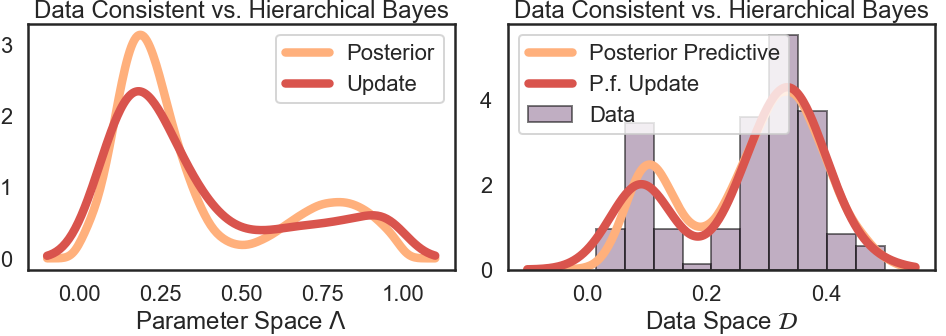
\includegraphics[width=30cm]{figures/distr_EX_comparison.png}
        \vspace{-0.5cm}
        \caption{ }
    \end{figure}
\end{block}
\heading{Non-parametric method with less sampling}
\heading{Future Research: How is it connected to Dirchlet Processes?}
